%!TEX root =  main.tex
\section{A New Test Statistic}\label{sec:f1}

In this section we describe our hypothesis test.  This begins with the introduction in Section \ref{subsec:f1def} of $F_1$, a new test statistic for the ANOVA setting.  In Section \ref{subsec:privf1} we then show how to privately compute a private approximation of $F_1$.  Finally, in Section \ref{subsec:alg-method} we calculate $p$-values for the private $F_1$ statistic.  This means simulating a correct reference distribution against which we can compare our output.


\subsection{The $F_1$ Statistic}\label{subsec:f1def}


Our goal is to define a statistic that releases similar information as the $F$-statistic, but has higher power (Definition~\ref{def:power}) for reasonable privacy guarantees.  We focused on two approaches to improve the power of the ANOVA calculation: reducing the amount of Laplacian noise by decreasing sensitivity, and making \ssa and \sse numerically larger so that the noise has less influence over the total value of the statistic.  We achieved both goals by taking the absolute values of the summand terms in the \ssa and \sse, rather than squaring them. 

% old text
%We are looking for a new test statistic that provides similar information about a database as the $F$-statistic, but that has higher power. The main issue with the differentially private $F$-test is that it requires thousands of data points to reach full power even for $\eps = 1$, a modest privacy guarantee. 
%There are many ways one could potentially try to improve the power of the ANOVA calculation. We focused on two approaches: decreasing sensitivity and increasing the numerical size of the statistic. The sensitivity of the \ssa and \sse determine the amount of Laplacian noise that is added to the private \ssa and \sse. Thus, one way to improve the power of the ANOVA calculation is to create a statistic that has lower sensitivity. An additional improvement to ANOVA is making the \ssa and \sse numerically larger so that the noise has less influence over the total value of the statistic.
%We achieved both of these goals by taking the absolute values of the summand terms in the \ssa and \sse rather than squaring them. We call these modified statistics \sa and \se, defined below. First, the sensitivities of \sa and \se are less than half as large as the sensitivities of \ssa and \sse. In addition, taking the absolute value rather than squaring terms yields a larger statistic because the terms of the summand are restricted to the interval $[0,1]$. 
%This modified $F$-statistic measures within-group variance compared to between-group variance in essentially the same way as the original $F$-statistic. The \sa is zero when calculated on null data (data where the group means are all equal), but it grows as the group means diverge from one another. Thus, we want to reject the null hypothesis when the means are far apart. The \se provides a sense of scale for how far the means have diverged.

%\subsection{Our test}
As before, let \k denote the number of categories in the database, $c_i$ be the category and $y_i$ be the numerical value associated with observation $i$, $n_j$ be the size of category $j$, and $N$ be the total size of the data set. Additionally, $\bar{y}$ is the grand mean of the entries in database \x and $\bar{y}_j$ is the mean of the entries in group $j$. 
\begin{definition}[$F_1$-statistic]\label{def:f1stat}
Given a database \x with $k$ groups and \dbsize total entries, the $\sa(\x)$ and $\se(\x)$ calculations are defined as follows:
\begin{align*}
\sa(\x)  &= \sum_{j = 1}^{k} n_{j} \lvert \bar{y} - \bar{y}_{j} \rvert \\
\se(\x) &= \sum_{i=1}^N \lvert y_{i} - \bar{y}_{c_i} \rvert.
\end{align*}
The $F_1$-statistic is the ratio of \sa and \se, each divided by their respective degrees of freedom. 
\begin{equation*}
F_1(\x) = \frac{\sa(\x)/(k-1)}{\se(\x)/(\dbsize-k)}.
\end{equation*}
\end{definition}

The $F_1$-statistic measures variation between group means compared to variation within groups in essentially the same way as the original $F$-statistic. The \sa grows as the group means diverge.  What constitutes a ``large'' variation between group means depends on the variation between individual items, so \se, which measures this individual-level variation, provides a sense of scale for the \sa value.


In the next section, we show that the sensitivities of \sa and \se in the $F_1$-statistic are less than half as large as the sensitivities of \ssa and \sse in the original $F$-statistic. Further, because the summand terms are restricted to $[0,1]$, the \sa and \se values are much larger, meaning they can tolerate the addition of more noise before losing their usefulness.

\subsection{A Private Approximation of $F_1$}\label{subsec:privf1}

The sensitivity of $F_1$ is very high.  (In the worst case, $\se(\x)$ is almost zero and very small changes can have huge effects on $F_1(\x)$.)  As a result, we can't simply apply the Laplace mechanism to $F_1$.  Instead, we choose to apply it individually to the \sa and \se functions, and then use composition and post-processing to compute an estimate of $F_1$.  We must therefore bound the sensitivities of \sa and \se.

We assume that the number of valid category values, \k, is fixed and public, but the number of entries in each group is not.  (This includes the possibility that one or more categories exist as valid entries but do not appear in the actual database.)   We also assume that there are maximum and minimum possible values for the data, and that the computation first uses these to normalize the data, mapping it to the interval $[0,1]$.

\begin{theorem}[SE Sensitivity] \label{thm:SEsens}
The sensitivity of the \se calculation in Definition~\ref{def:f1stat} is bounded above by 3.
\end{theorem}

\begin{proof}

Suppose neighboring databases \x and \xprime differ by some row $r$ in both the categorical and numerical values. Say that in \x, $c_r = a$, and in \xprime, $c_r = b$. Note that this change will lead to a larger difference in the calculation of the \se than the difference would be if the categorical variable did not change. Let $n_a$ be the size of category $a$ excluding $r$ and let $n_b$ be the size of category $b$ excluding $r$. We begin by expressing the \se calculation as nested summations indexing over group size and entries within each group.

$$ \se(\x) = \sum_{j=1}^k \sum_{i \in C_j}  \lvert y_{i} - \bar{y}_{c_i} \rvert. $$

Call $t_{i} = \lvert y_{i} - \bar{y}_{c_i} \rvert$, and let $c_i \neq a,b$. Then, $t_{i}$ does not change between \x and \xprime. Now, suppose $i \ne r$ but $c_i = a$. It follows that $\Delta t_{i} \le 1/(n_a+1)$, since the only change comes from $\bar{y}_{a}$. There are $n_a$ such terms, so the total contribution from these terms is at most $n_a/(n_a+1)$. Similarly, if we consider $t_{i}$ where $i \ne r$ but $c_i = b$, $\Delta t_{i} \le 1/(n_b+1)$. Thus, the terms in groups $a$ and $b$ excluding row $r$ together contribute 
$$ \frac{n_a}{n_a+1} + \frac{n_b}{n_b+1} \leq 2.$$

Now, consider $\Delta t_{r}$. Since $y_{r}$, $\bar{y}_{a}$, and $\bar{y}_b$ are all in the interval $[0,1]$, the difference between $t_{r}$ in database \x and in \xprime is at most 1. Thus, the total sensitivity of \se is bounded above by 3.

\end{proof}


\begin{theorem}[SA Sensitivity] \label{thm:SAsens}
The sensitivity of the SA calculation in Definition~\ref{def:f1stat} is bounded above by 4. 
\end{theorem}

\begin{proof}
Again, suppose neighboring databases \x and \xprime differ by some row $r$ in both the categorical and numerical values, with $c_r = a$ in \x, and $c_r = b$ in \xprime. Denote the number of entries in groups $a$ and $b$ not including row $r$ by $n_a$ and $n_b$, respectively. We begin by expressing the \sa calculation as two sums indexing over groups and entries within each group.
$$
\sa(\x)  = \sum_{j = 1}^{k}\sum_{i \in C_j} \lvert \overline{y} - \overline{y}_{c_i} \rvert
$$

Consider the change from $\sa(\x)$ to $\sa(\xprime)$ as if it occurred in two steps.  In the first step, the grand mean $\overline{y}$ is updated.  Note that in the worst case, $\bar{y}$ can change by at most $1/\dbsize$ between \x and \xprime. Then, since there are $N$ summands, each including the grand mean, this step changes the value by a maximum of $N(1/N)=1$ to the overall sensitivity. 

In the second step we change the group means for groups $a$ and $b$.  There will be $n_a$ terms containing $\overline{y}_a$, each of which will change by at most $1/n_a$, changing the overall value by at most 1.  Similarly updating $\overline{y}_b$ changes $n_b$ terms each by at most $1/n_b$ for a total contribution of 1.  

%When $i\in C_a$, the group mean will change as well, and has sensitivity bounded above by $1/n_a$. Then, excluding $r$, there are $n_a$ terms who will contribute $1/n_a$ to the sensitivity, and thus $\overline{y}_a$ contributes a maximum of $n_a(1/n_a)=1$ to the overall sensitivity. Similarly, $\overline{y}_b$ contributes a maximum of $n_b(1/n_b)=1$ to the overall sensitivity. 

Finally, the change of $r$ between \x and \xprime contributes 1 to the overall sensitivity, and thus the sensitivity of the \sa is bounded above by 4.
%
%Consider the $t_i$ where $c_i\neq a,b$. For each term, $\bar{y}_{c_i}$ is the same in \x and \xprime, thus the sensitivity of is bounded above by $1/\dbsize$. Thus, the total contribution to the \sa sensitivity from rows in groups unaffected by row $r$ is 
%
%$$1/N \cdot (\dbsize - (n_a + n_b + 1)) = 1 - \frac{n_a + n_b + 1}{\dbsize} \leq 1.$$ 
%
%\ab{In this section we're treating the $t_r$ the same as all other $t_i$ where $c_i = a, b$. It's not clear to me why we can do that. For those $t_i$ where $c_i = a$, the term goes from $\lvert \bar{y} - \bar{y}_a \rvert$ to $\lvert \bar{y} - \bar{y}_a \rvert$ where both the grand mean and the group mean have changed. For $t_r$, the term goes from $\lvert \bar{y} - \bar{y}_a \rvert$ to $\lvert \bar{y} - \bar{y}_b \rvert$. We need to provide an explanation for why we can treat those the same way.}
%\igh{Fixed it?} Next, consider the $t_i$ where $c_i=a$. It follows that $\bar{y}_{c_i}$ can change by at most $1/(n_{a}+1)$. Thus, $\Delta t_i \le 1/\dbsize + 1/(n_a+1)$. The same holds when $c_i = b$. Then, the contribution of the terms in groups $a$ and $b$ excluding $r$ is
%\begin{align*}
%n_a \left( \frac{1}{\dbsize} + \frac{1}{n_a+1}\right) + n_b \left( \frac{1}{\dbsize} + \frac{1}{n_b+1} \right)
%&= \frac{n_a}{\dbsize} + \frac{n_a}{n_a+1} + \frac{n_b}{\dbsize} + \frac{n_b}{n_b+1}  \\
%&= \frac{n_a+n_b}{\dbsize}  + 1  + \frac{n_b}{n_b+1} \\
%&\leq 1+1+1\\
%&=3.
%\end{align*}
%\indent Then, since the contribution of $r$ is bounded by 1, the total sensitivity of \sa is bounded above by 4. 
\end{proof}


Having proven these sensitivities, we can now introduce our private algorithm (Algorithm \ref{alg:F1}) for approximating $F_1$.  The algorithm first estimates \sa and \se, allocating part of the privacy budget to each one. We introduce a parameter $\rho \in (0,1)$ that determines the relative amount of the privacy budget spent on each intermediate value.  The optimal value of $\rho$ will be experimentally determined in Section \ref{subsec:optrho}.  We note that in addition to using a different test statistic, the prior work by Campbell et al.~did not consider $\rho$ values other than 0.5.

\begin{algorithm}
%Note: label has to be inside caption or else it will refer to subsection number instead of algorithm number
    \caption{private\_F1($\x,\eps, \rho$) \label{alg:F1}}
    \begin{algorithmic}
        %\STATE \textbf{Input:} Database $\x$, $\eps$ value
	%\STATE \textbf{Output:} $\widehat{F_1}, \widehat{\text{SA}}, \widehat{\text{SE}}$
        \STATE $\widehat{\text{SA}} = \text{SA}(\x) + L_1$ where $L_1\sim\text{Lap}\left(\frac{4}{\rho\eps}\right)$ 
        \STATE $\widehat{\text{SE}} = \text{SE}(\x) + L_2$ where $L_2\sim\text{Lap}\left(\frac{3}{(1-\rho)\eps}\right)$
        \STATE  $\widehat{F_1} = \frac{\widehat{\text{SA}}/(k-1)}{\widehat{\text{SE}}/(N-k)}$
        \STATE return $\widehat{F_1}, \widehat{\text{SA}}, \widehat{\text{SE}}$
    \end{algorithmic}
\end{algorithm}

\begin{theorem} \label{thm:AlgPriv}
Algorithm \ref{alg:F1} is \eps-differentially private.
\end{theorem}
\begin{proof}
By the sensitivity bounds of \se and \sa in Theorems \ref{thm:SEsens} and \ref{thm:SAsens}  and the Laplace mechanism (Theorem \ref{thm:lapmechanism}), $\widehat{\sa}$ is $\rho\eps$-differentially private and $\widehat{\se}$ is $(1-\rho)\eps$-differentially private. By the composition theorem (Theorem \ref{thm:composition}), outputting both is \eps-differentially private. Since $k$ and \dbsize are both public information, computing $\widehat{F_1}$ is post-processing (Theorem \ref{thm:postprocessing}).
\end{proof}


\subsection{Reference Distribution and $p$-values}
\label{subsec:alg-method}


As discussed previously, the test statistic on its own is not useful; we need a $p$-value to provide a sense of scale in the context of the null hypothesis. Computing a $p$-value begins with an accurate reference distribution.  We numerically approximate this distribution through simulation.  The intermediate values of the $F$ statistic, \ssa and \sse, are drawn from  $\sigma^2\chi_{k-1}^2$ (for \ssa) and $\sigma^2\chi_{n-k}^2$ (for \sse).  Campbell et al.~used this to easily sample from the correct distributions for \ssa and \sse.

The \sa and \se values needed to compute $F_1$ follow no similarly tractable distribution, so instead we simulate full databases according to the null hypothesis and for each calculate $\widehat{F_1}$.  The distribution of these $\widehat{F_1}$ values approximates the reference distribution.  The goal, given a database \x, is to simulate databases with the same size $N$ and number of groups $k$, same standard deviation $\sigma$, and same expected value $\mu$.  The values $N$ and $k$ are public, so we can use those values.  The expected value $\mu$ is not, but as long as it is safely inside the $[0,1]$ interval, its value has no effect on the distribution, so we simply always use 0.5. 


%The method we used to calculate the $p$-value for a given $\widehat{F_1}$-statistic differs from prior work. While Campbell et al.~used the fact that under the null hypothesis, the \ssa is drawn from $\sigma^2\chi_{k-1}^2$ and \sse is drawn from $\sigma^2\chi_{n-k}^2$, we do not have a similar luxury for \sa and \se.

%Instead, we simulate full databases to get the distribution of the $\widehat{F_1}$-statistic and compute the $p$-value. Given the input database \x, we simulate databases with the same standard deviation and same size as \x, but that share the same mean across the groups. This mean could conceivably be any value in the unit interval; we set it to .5 to limit the amount of clipping caused when the data is rescaled. For each of the null databases, we compute the $\widehat{F_1}$-statistic using Algorithm~\ref{alg:F1} for an empirical approximation fo the distribution of the $\widehat{F_1}$-statistic under the null hypothesis.

Unfortunately, using an accurate $\sigma$ is more difficult.  Unlike in the non-private setting, the reference distribution depends on the choice of $\sigma$, so an inaccurate value can cause incorrect results.  We had two choices: either we could use some of our \eps-budget to directly estimate the standard deviation of the $y_i$ in database \x (see Appendix~\ref{Sec:AppDirSig}), or we could devise an indirect method of estimating the standard deviation given $\widehat{\sa}$ and $\widehat{\se}$. We focused on the latter by deriving an unbiased estimator $\hat{\sigma}$ for $\sigma$.

$$
\hat{\sigma} = \frac{\widehat{SE}}{\tilde{N}}\sqrt{\frac{\pi}{2}}, \text{ where } \tilde{N} = \sum_{j=1}^k n_j \sqrt{\left(1 - \frac{1}{n_j}\right)}
$$

See Appendix \ref{Sec:AppSig} for the proof that this is indeed an unbiased estimator.  

Computing this estimator requires knowledge of each of the group sizes, which are private. Fortunately, $\tilde{N}$ is closely approximated by $N-k$, which we know. At the smallest database sizes that we considered (around $N = 100$ with three equal-sized groups), this approximation has < 1\% error. As the size of the database grows, this error shrinks to zero.  Figure \ref{fig:sigma-estimate} visualizes the unbiasedness and asymptotically shrinking variance of $\hat{\sigma}$. (using the $\tilde{N} = N-k$ approximation).  We further confirm in Section 4 that it is precise enough to compute valid $p$-values. 


\begin{figure}
\centering
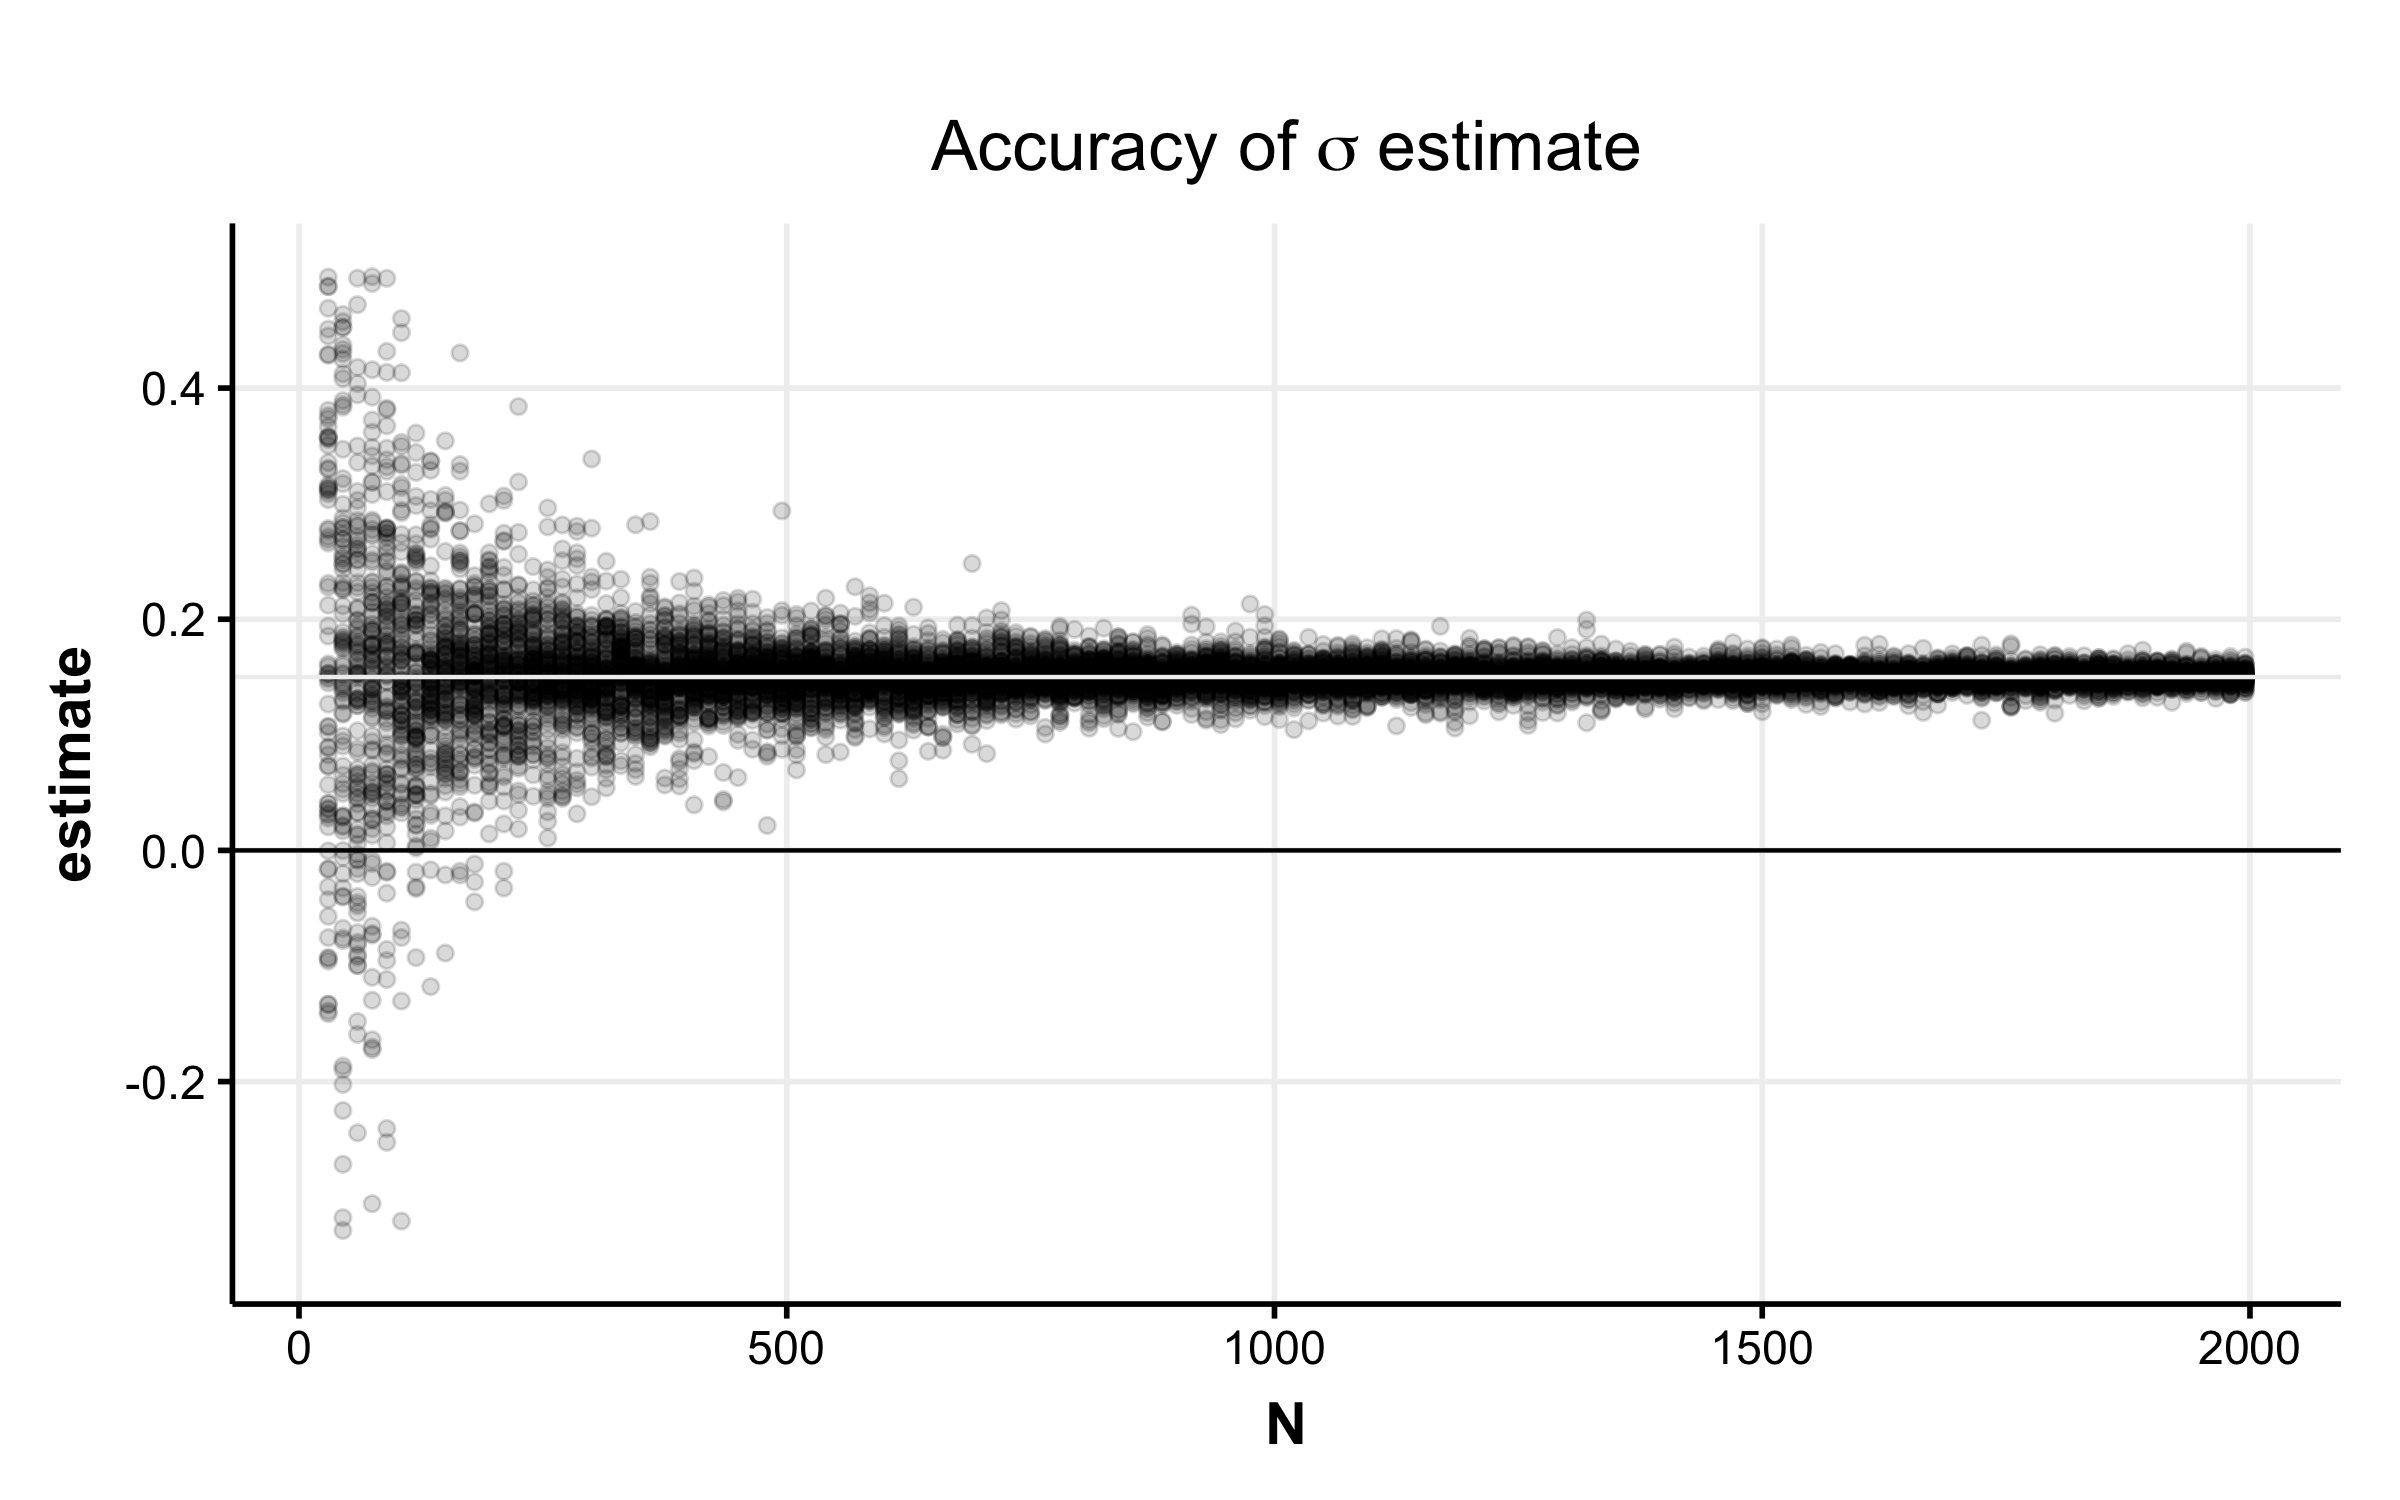
\includegraphics[width=\linewidth]{sigma-estimate.png}
\caption{$\hat{\sigma}$ is unbiased ($\sigma = .15$) with shrinking variance as N grows large. Each point represents the estimate from a simulated null database. At small N, there is a non-zero probability of returning a negative estimate.\label{fig:sigma-estimate}}
\end{figure}

Another issue presented by the private estimation of $\sigma$ is that the Laplacian noise can be large enough to make the estimate negative. Negative standard deviation estimates are more likely to occur when the \se is small, i.e.~when the database is small or when the within-group standard deviation is small.

This problem is unique to the private setting and we do the most conservative possible thing --- we never reject the null hypothesis when the estimated standard deviation was negative. Our reasoning was that a negative standard deviation has no statistical meaning and any calculations made from such an estimate would be uninformative.  This method for dealing with negative standard deviation estimates results in a type I error rate lower than $\alpha$, which means that our results are more conservative. As was mentioned earlier, the \sa increases as the database size and effect size between groups increases. Thus, negative standard deviation estimates tend to occur for database sizes and effect sizes that are so small that the effect is undetectable anyway.  As a result, this conservative choice does little to reduce the power of our test.

A formal description of the private $F_1$ ANOVA test in presented in Algorithm~\ref{alg:pval}, which returns a Boolean indicating whether the null hypothesis $H_0$ is rejected. Note that Algorithm~\ref{alg:pval} only accesses the data through a call to Algorithm~\ref{alg:F1}, and Algorithm~\ref{alg:F1} is already shown to be private, therefore the privacy of Algorithm~\ref{alg:pval} follows immediately from Theorem~\ref{thm:postprocessing}.
\begin{algorithm}
%Note: label has to be inside caption or else it will refer to subsection number instead of algorithm number
    \caption{ANOVA\_test($\x$, $\eps$, $\alpha$, \emph{reps})\label{alg:pval} }
    \begin{algorithmic}
        %\STATE \textbf{Input:} Database $\x$, $\eps$ value, $\alpha$ significance level, \emph{reps} iterations
        \STATE $\widehat{F_1}, \widehat{\sa}, \widehat{\se} =$ private\_F1($\x$,$\eps$)
        \IF{$\widehat{\text{SE}}<0$}
        \STATE return \text{False}
        \ENDIF
        \STATE $\widehat{\sigma} = \sqrt{\pi/2}\frac{\widehat{\text{SE}}}{(\dbsize-k)}$
        \STATE $significant = 0$
        \FOR{$i = 1$ to \emph{reps}}
        \STATE  $\x^{ref} = N$ draws from $\normal(0.5, \widehat{\sigma})$ divided into $k$ equal-sized groups
        \STATE $\widehat{F_1}^{ref}, \widehat{\sa}^{ref}, \widehat{\se}^{ref} =$ private\_F1($\x^{ref}, \eps$)
        \IF{$\widehat{F_1}^{ref} > \widehat{F_1} $}
        \STATE $significant = significant + 1$
        \ENDIF
        \ENDFOR
        \STATE $p$-value $= significant/reps$
        \IF{$p$-value $< \alpha$}
        \STATE return \text{True}
        \ELSE 
        \STATE return \text{False}
        \ENDIF
    \end{algorithmic}
\end{algorithm}

% \begin{figure}
% \centering
% 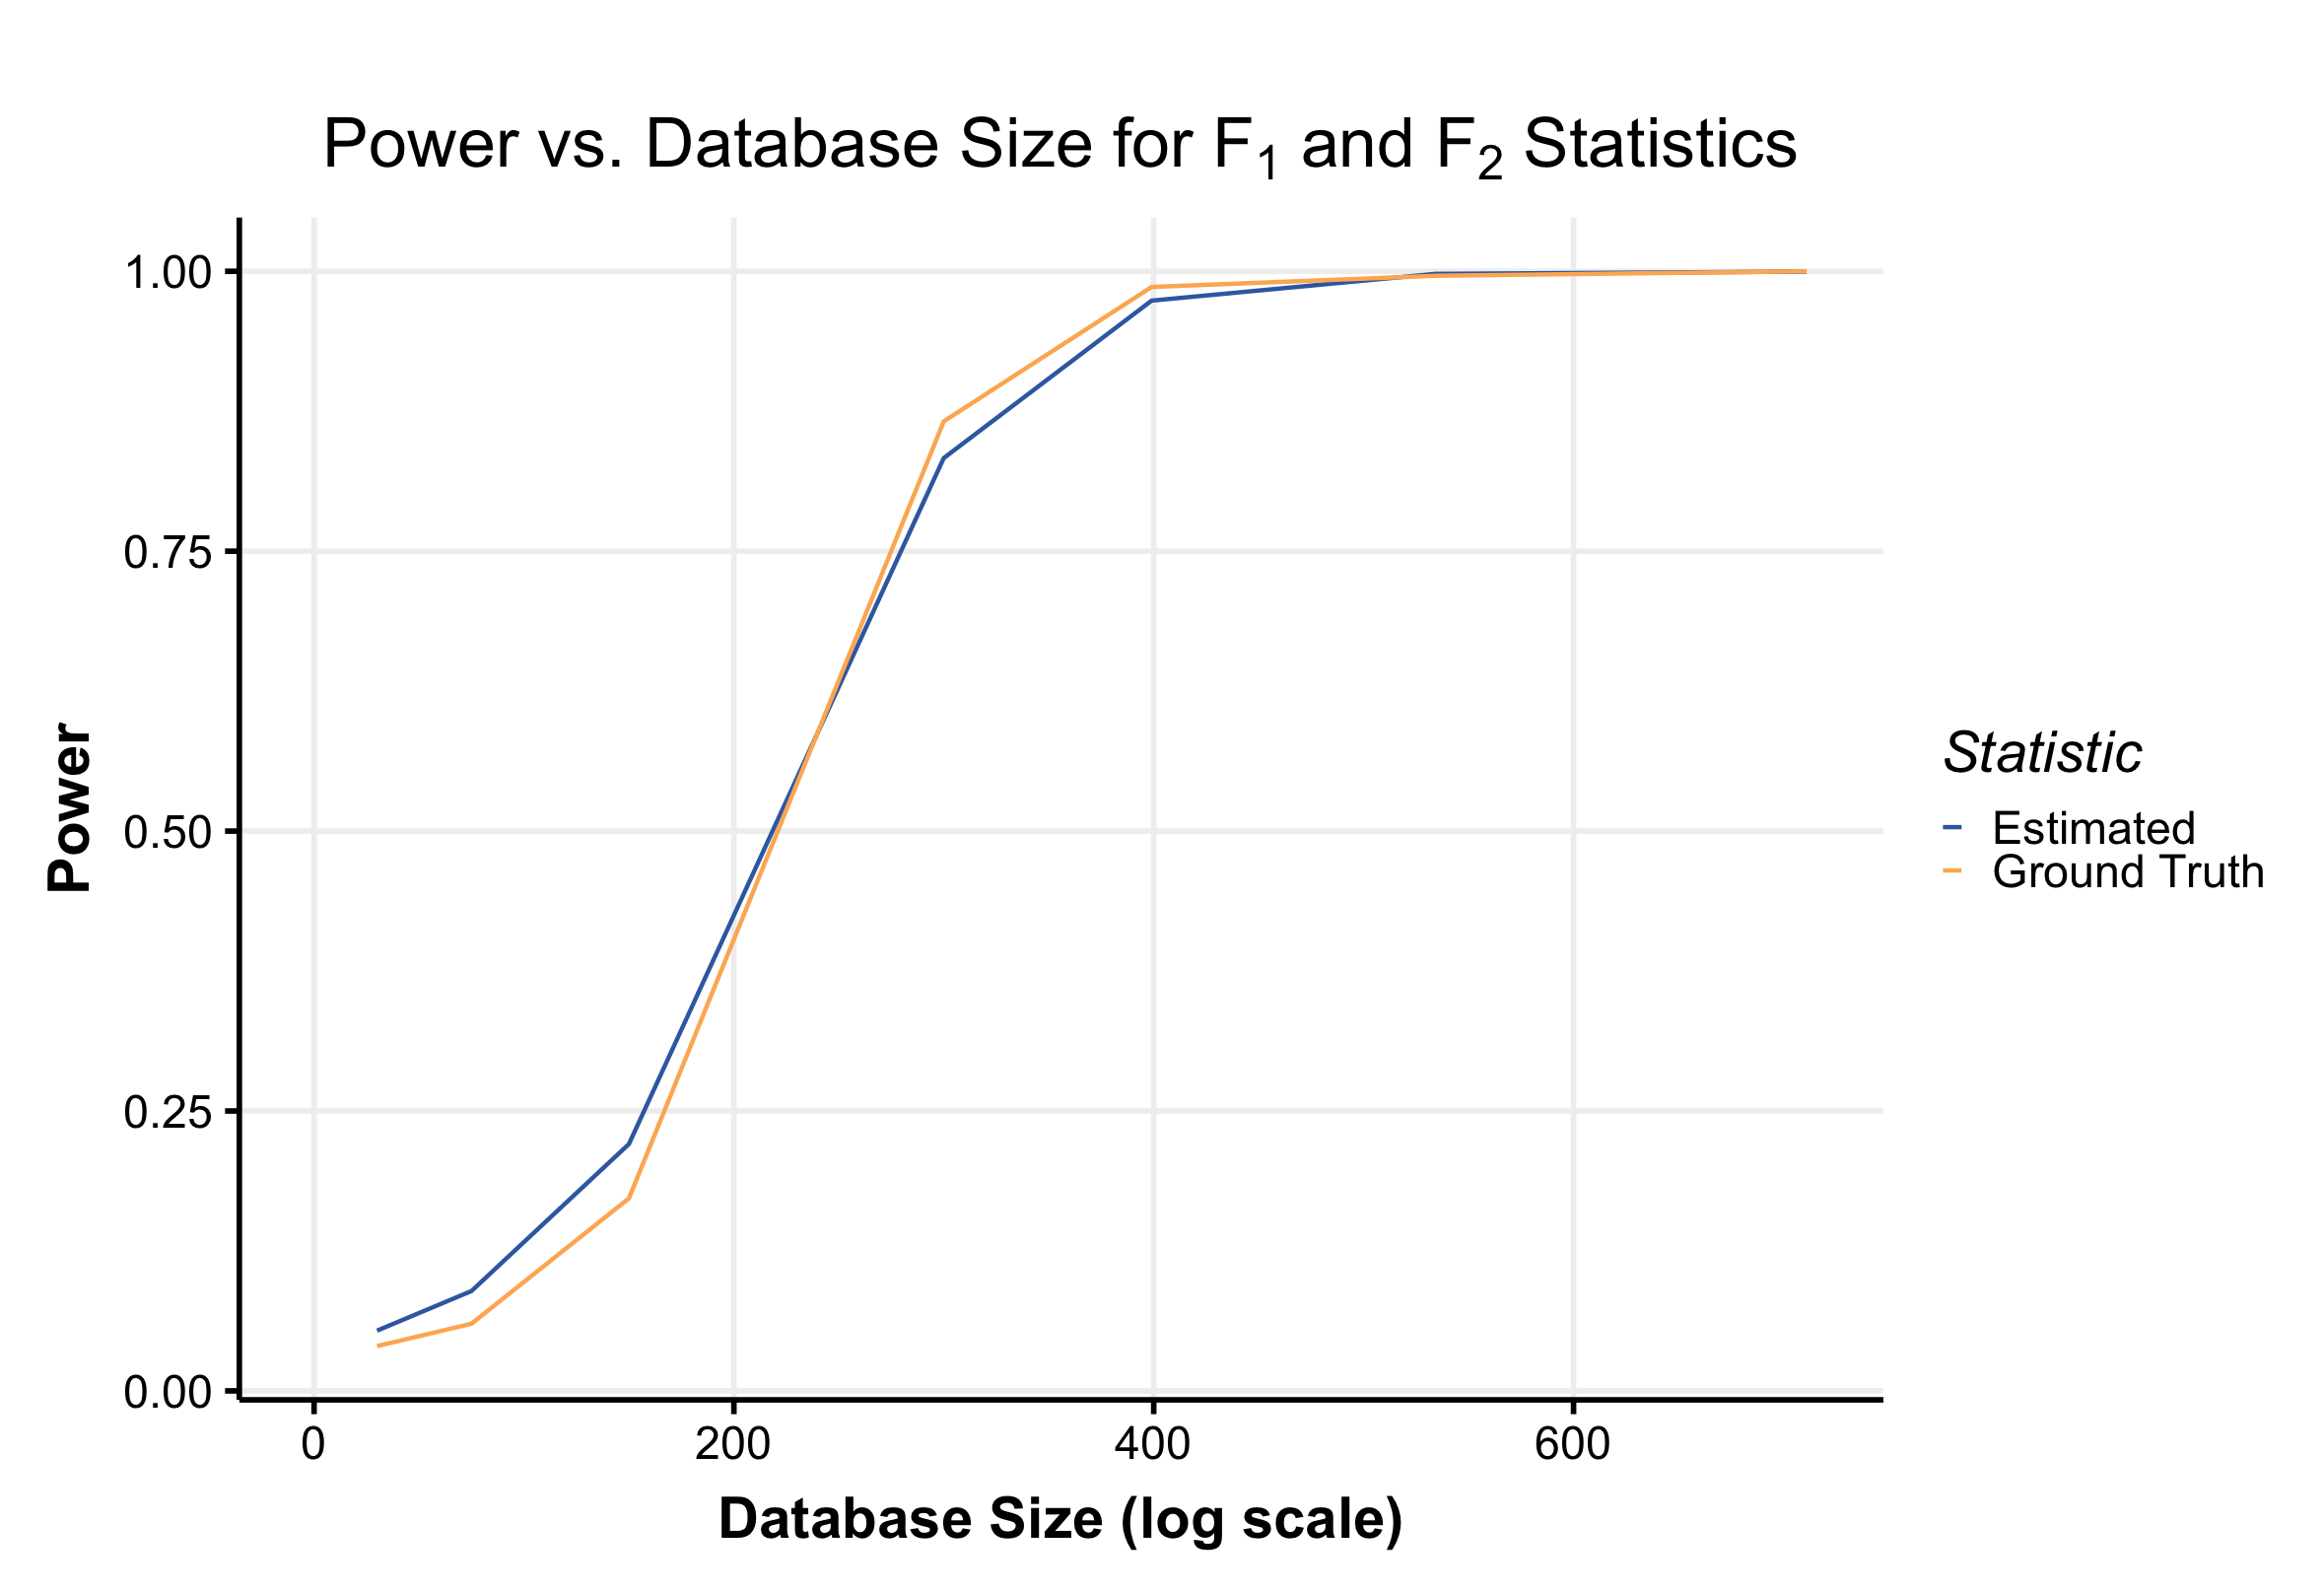
\includegraphics[width=\linewidth]{estvar-vs-truevar.png}
% \caption{Hypothesis tests conduced by estimating $\sigma$ yield comparable power with tests using ground truth $\sigma$. $\varepsilon$ = 1.}
% \end{figure}
